

\section{Introduction}
To begin the discussion of high dimensional probability, we ought to review some basic principles of probability. Many of the results that we discuss in this course will lean heavier on moment generating functions than in introductory courses. As a consequence, we shall dive into the intuition of moment generating functions. 

Since high-dimensional probability begins with a discussion of concentration inequalities, we will also take the time to review some basic inequalities in order to make sure our tools are sharp. 
\subsection{Moment Generating Functions (MGFs)}
\begin{tcolorbox}
\begin{definition}[Moment Generating Function]
    Let $t \in \mathbb{R}.$ If it exists around the neighborhood $t=0$, we define the moment generating function of the RV $X$ as 
    \begin{equation}
    M_X(t) = E\left[e^{tX}\right] 
    \end{equation}
\end{definition}
\end{tcolorbox}


Moment generating functions are important theoretical objects in probability theory. Primarily, they are important because they can uniquely characterize a probability distribution and allow us to easily obtain the $n$th moment of any distribution. In a sense, they capture the "soul" of a probability distribution. To understand the underlying mathematical machinery of moment generating functions further, notice that the MGFs can be represented as follows:

% Equation
\begin{align*}
    M(t) &= E[ e^{tX} ]     \\ 
    &= E\left[ 1 + tX + \frac{t^2 X^2}{2!} + ... + \frac{t^n X^n}{n!} + ...\right] && \text{series expansion}\\
    &= E\left[ 1 \right] + E\left[tX\right] + E\left[\frac{t^2 X^2}{2!}\right] + ... + E\left[\frac{t^n X^n}{n!}\right]+... &&\text{property of expectation} \\
    &= 1 + tE[X] + \frac{t^2}{2!}E[X^2] + ... + \frac{t^n}{n!} E[X^n] + ...
\end{align*}

\noindent Now, with the expanded form of the MGF, we can easily obtain the $n$th moment of the random variable $X$. The following box summarizes this procedure succintly, and Figure \ref{fig:MGF} illustrates the intuition. \\

\begin{tcolorbox}[colback=white!90!gray, title=Intuition: Find the $n$th moment of $X$]
\begin{enumerate}
    \item expand series $E[e^{tX}]$
    \item take the $n$th derivative
    \begin{itemize}
        \item the first $(n-1)$ terms go to 0 
    \end{itemize}
    \item set $t=0$
    \begin{itemize}
        \item terms $(n+1), (n+2), ...$ go to 0
    \end{itemize}
\end{enumerate}
\end{tcolorbox}

% Illustration of MGF
\begin{figure}[H]
\centering
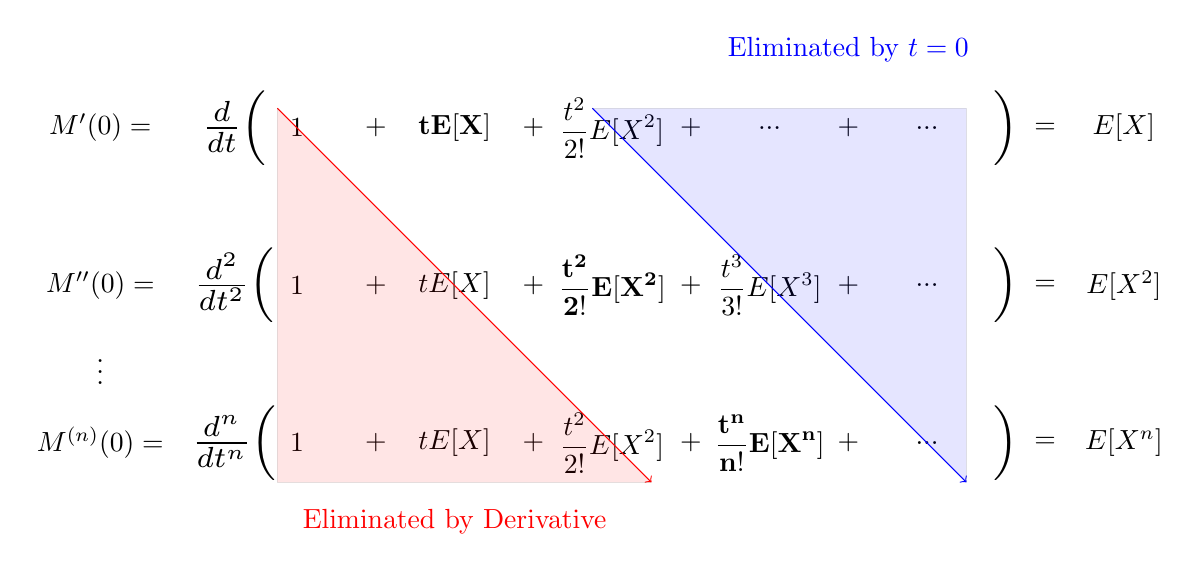
\begin{tikzpicture}

    % 1st Row 
    % -------
    \node[] (10) at (0,0) {1};        
    \node[] (11) at (2,0) {$\mathbf{\displaystyle{tE[X]}}$};  
    \node[] (12) at (4,0) {$\displaystyle{\frac{t^2}{2!}E[X^2]}$}; 
    \node[] (1k) at (6,0) {$...$}; 
    \node[] (1n) at (8,0) {$...$}; 
    \node[] (1n) at (10.5,0) {$E[X]$}; 
    
    \node[] at (1,0) {$+$};
    \node[] at (3,0) {$+$};
    \node[] at (5,0) {$+$};
    \node[] at (7,0) {$+$};
    \node[] at (9.5,0) {$=$};
    
    % 2nd Row 
    % -------
    \node[] (20) at (0,-2) {1};        
    \node[] (21) at (2,-2) {$\displaystyle{tE[X]}$};  
    \node[] (22) at (4,-2) {$\mathbf{\displaystyle{\frac{t^2}{2!}E[X^2]}}$}; 
    \node[] (2k) at (6,-2) {$\displaystyle{\frac{t^3}{3!}E[X^3]}$}; 
    \node[] (2n) at (8,-2) {$...$}; 
    \node[] (1n) at (10.5,-2) {$E[X^2]$}; 
    
    \node[] at (1,-2) {$+$};
    \node[] at (3,-2) {$+$};
    \node[] at (5,-2) {$+$};
    \node[] at (7,-2) {$+$};
    \node[] at (9.5,-2) {$=$};
    
    % 3rd Row 
    % -------
    \node[] (30) at (0,-4) {1};        
    \node[] (31) at (2,-4) {$\displaystyle{tE[X]}$};  
    \node[] (32) at (4,-4) {$\displaystyle{\frac{t^2}{2!}E[X^2]}$}; 
    \node[] (3n) at (6,-4) {$\mathbf{\displaystyle{\frac{t^n}{n!}E[X^n]}}$}; 
    \node[] (3k) at (8,-4) {$...$}; 
    \node[] (1n) at (10.5,-4) {$E[X^n]$}; 
    
    \node[] at (1,-4) {$+$};
    \node[] at (3,-4) {$+$};
    \node[] at (5,-4) {$+$};
    \node[] at (7,-4) {$+$};
    \node[] at (9.5,-4) {$=$};
    
    % Draw Paths 
    % ----------
    \draw[red , ->] (-0.25,0.25) -- ( 4.5,-4.5);
    \draw[blue, ->] ( 3.75,0.25) -- ( 8.5,-4.5);
    \draw[fill=red,opacity=0.1] (-0.25,0.25) -- (-0.25,-4.5) -- (4.5,-4.5);
    \draw[fill=blue,opacity=0.1] ( 3.75,0.25) -- ( 8.5,0.25) -- (8.5,-4.5);
    
    % Labels
    % ------
    \node[red]  at (2,-5) {Eliminated by Derivative};
    \node[blue] at (7, 1) {Eliminated by $t=0$};
    \node[] at (-2.5, 0) {$M'(0)=$};
    \node[] at (-2.5,-2) {$M''(0)=$};
    \node[] at (-2.5,-3) {$\vdots$};
    \node[] at (-2.5,-4) {$M^{(n)}(0)=$};
    
    \node[scale=1.5] at (-0.8, 0) {$\frac{d}{dt}\Big($}; 
    \node[scale=1.5] at (-0.8,-2) {$\frac{d^2}{dt^2}\Big($}; 
    \node[scale=1.5] at (-0.8,-4) {$\frac{d^n}{dt^n}\Big($}; 
    \node[scale=1.5] at (9, 0) {$\Big)$}; 
    \node[scale=1.5] at (9,-2) {$\Big)$}; 
    \node[scale=1.5] at (9,-4) {$\Big)$}; 
    
\end{tikzpicture}
\label{fig:MGF}
\caption{Illustration of Obtaining $n$th Moment of $X$}
\end{figure}

